\documentclass[a4paper]{article}

\usepackage{amsmath}
\usepackage{amsfonts}
\usepackage{graphicx}
\usepackage{enumerate}
\usepackage{SIunits}
\usepackage{hyperref}
\usepackage{anysize}
\usepackage{hyperref}

\marginsize{2.5cm}{2.5cm}{1.5cm}{1.5cm}

\graphicspath{{./images/}}

\title{Design of Digital Platforms}
\author{Steven Janssens, Pieter Maene en Kristof Mari\"en}
\date{\today}

\begin{document}
\maketitle

\section{Overall Architecture}

After having written a software implementation of the Montgomery algorithm in \textit{C}, the conclusion was that this was too slow for a real implementation. Therefore, in the second part of this course, we made a hardware coprocessor that should significantly increase the speed. The final goal of this project was to build RSA encryption and decryption, a regularly used algorithm.\\

\begin{figure}[h]
	\center{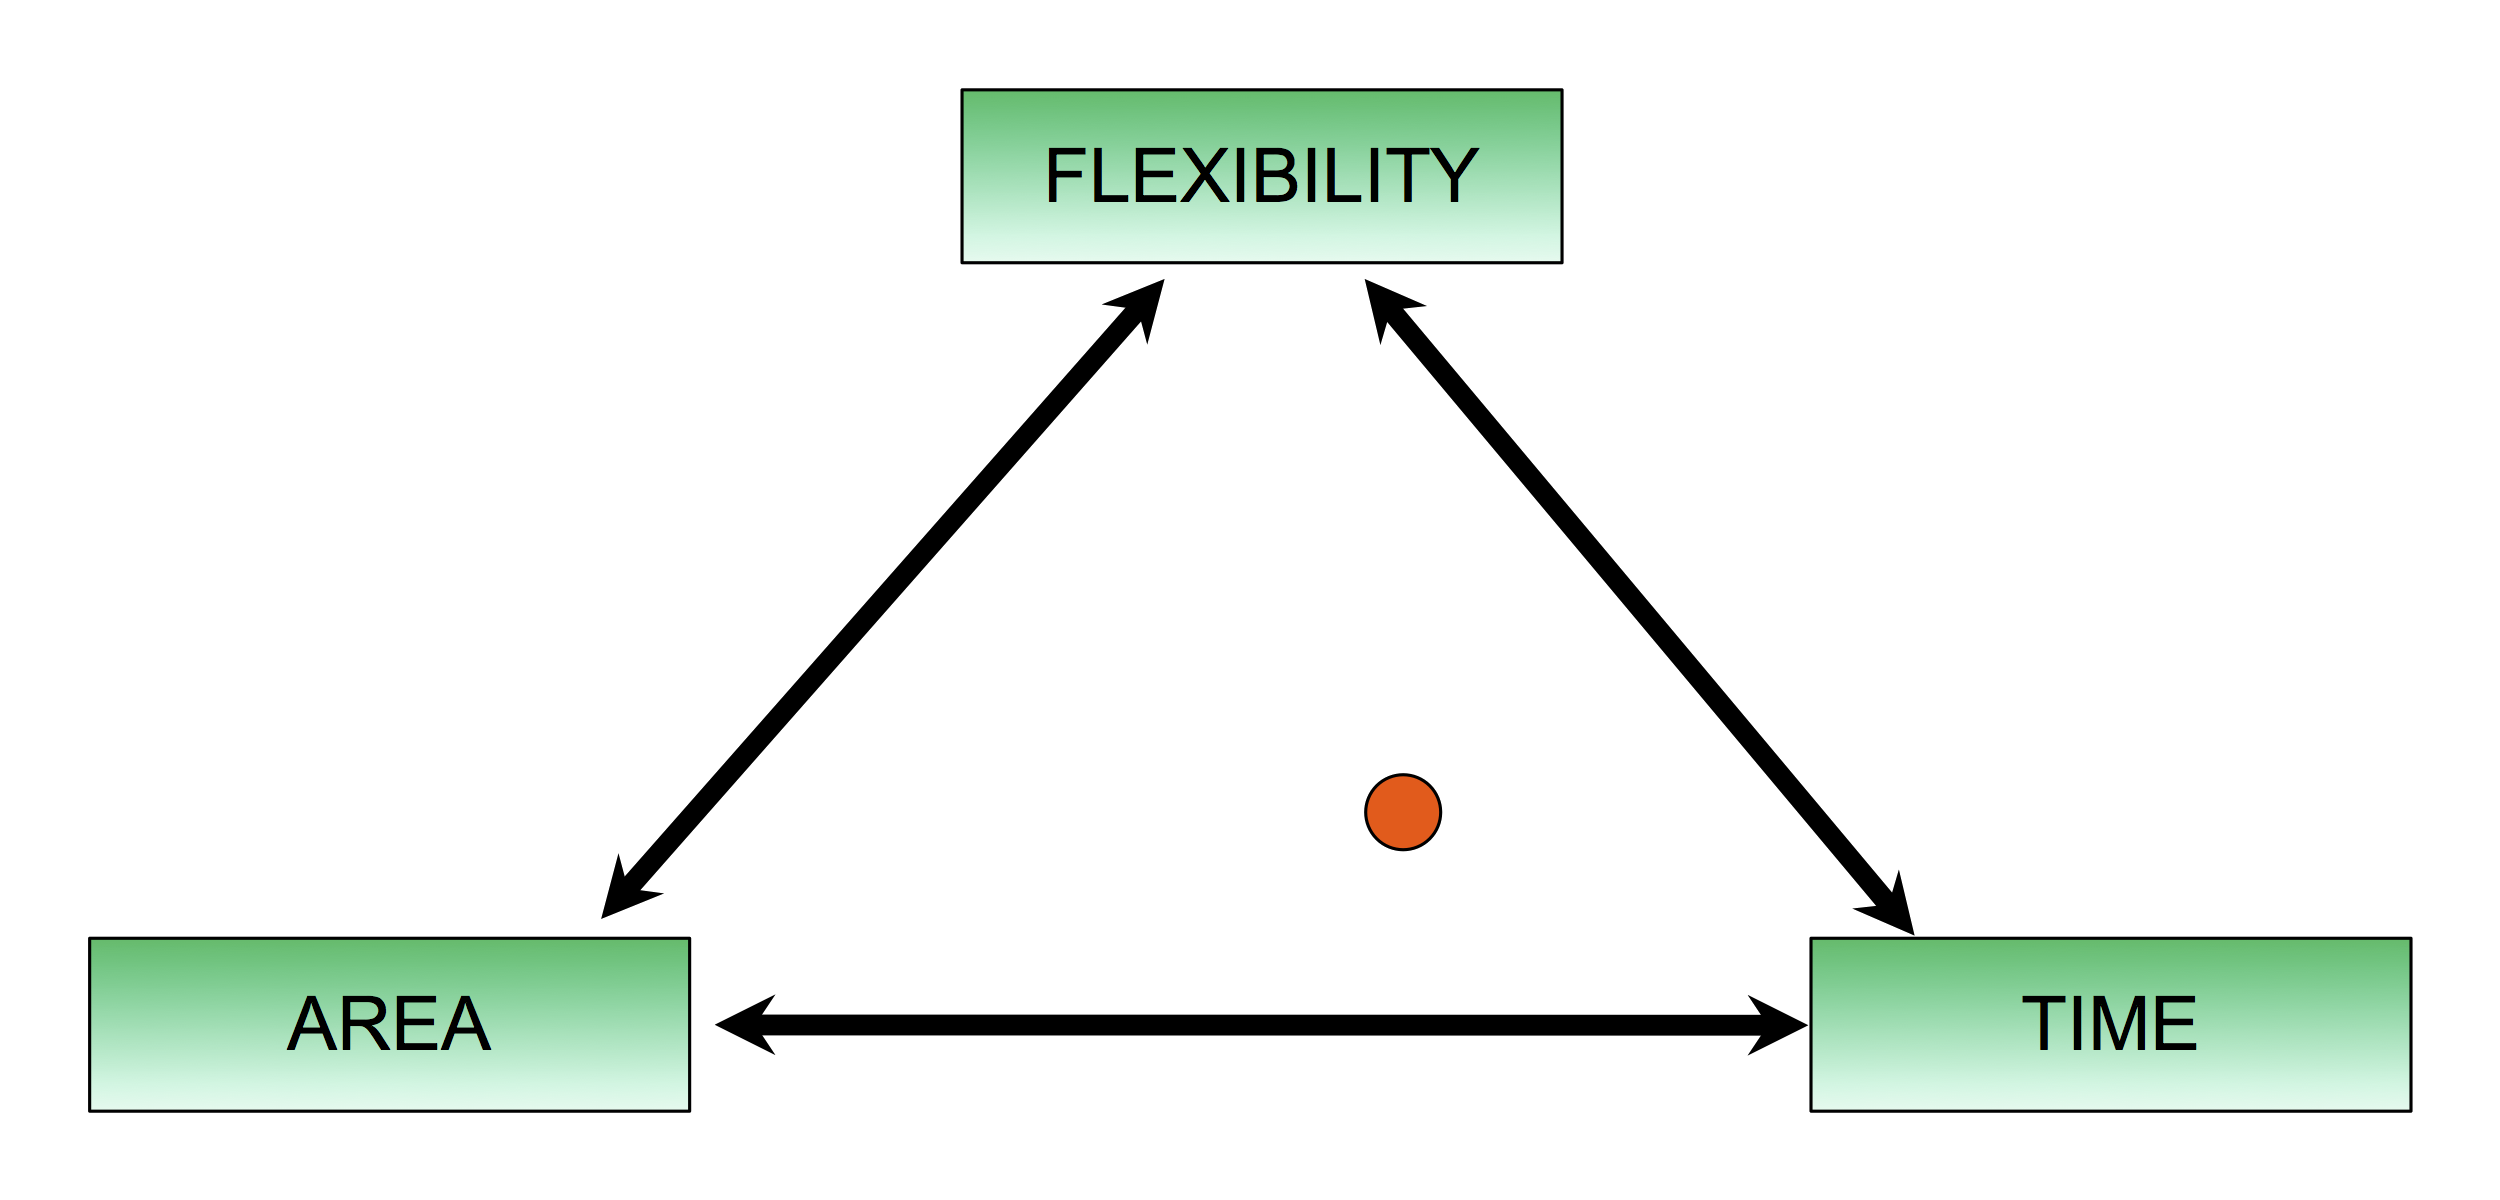
\includegraphics[width=0.8\linewidth]{situation.png}}
	\caption{Situation}
	\label{fig:situation}
\end{figure}

As you can see in Figure~\ref{fig:situation}, we decided to optimize our implementation towards time usage. Due to inherent design tradeoffs, this meant we had to sacrifice both flexibility and area. We made this choice because the only operation required by the RSA algorithm is an exponentation. So, we opted to build a coprocessor that was specifically designed to do a fast exponentiation. By implementing the exponentiation in hardware, there are some operations like shifting that make the algorithm a lot easier, which results in a faster implementation. However, there is still a datapath available that only computes one Montgomery multiplication. So a normal Montgomery multiplication can always be executed quite easily.\\

This hardware component could then be used in the software to implement the RSA encryption and decryption. This resulted in a two-way communication channel between the hardware and the software using the available I/O pins. To pass data back and forth, a memory-mapped implementation with a 2-way-handshake was chosen.

\section{HW/SW Boundaries}

The RSA algorithm is a basic and very often used algorithm for encryption and decryption of data. So it is important that the encryption and decryption is as fast as possible. The algorithm is standardized and will not change in the future. The only part of it that will change is the size of the inputs, as the encryption with larger numbers is more difficult to crack. Because of these facts a full hardware implementation was chosen.\\

From the previous section we know that a Montgomery multiplication implemented in \textit{C} takes about 1 second and a Montgomery exponentiation uses a lot of multiplications. So the multiplication must be done in hardware. Our hardware implementation of the multiplication takes about 1300 cycles. Assuming a clock frequency of about 5 \mega \hertz, this means a multiplication in hardware takes about 0,26 \micro \second.\\

So the only choice that was left, was to do the exponentiation in \textit{C} and call every time the Montgomery multiplication in the hardware or write the exponentiation in \textit{Gezel}. Doing the exponentiation in \textit{C} would cause a lot of overhead to transfer the data from the software to the hardware and back. So the benefits to write the exponentiation in \textit{Gezel} were quite obvious.

\section{HW/SW Interface}

For the communication between the hardware and the software a 2-way-handshake method is used. For passing the data from the software to the hardware the following procedure is followed. The software takes care of saving the data on the right places in the memory. If that is done, $P0$ is set to $ins\_write\_data$ to notify the hardware the data is available. The hardware immediately set $P1$ to one. After that the software loops (with an empty while loop), until the hardware sets $P1$ back to zero. If the software detects that the hardware has returned to an idle state, it notifies the detection to the hardware with an $ins\_ack$ on $P0$.\\

To pass the data from the software to the hardware, all the values are located after each other. So all the values form one block. In the hardware it was set how long each value is and so all the values are again separated. When the length of the inputs varies, this is where the changes have to be made.

\section{Performance Metrics}

The two measurable performance statistics are the number of registers used and the amount of clock cycles used for one computation of either the encryption or decryption. As the datapaths for encryption and decryption are equal, the amount of registers is the same in both as can be seen in Table~\ref{tab:performance metrics}. For the number of clock cycles there is clearly a difference between the encryption and the decryption. The decryption takes a lot more time because the decryption exponent is many times larger than the encryption exponent, so the amount of Montgomery multiplications increases with a big amount. This timing contains the reading of the input from the software (in the hardware), the Montgomery exponentiation itself and the writing back of the result from the hardware to the software.

\begin{table}[ht]
	\begin{center}	
		\begin{tabular}{c|c|c}
			 & \textbf{Encryption} & \textbf{Decryption}\\
			\textbf{Registers} & 12351 bit & 12351 bit\\
		 	\textbf{Clock cycles} & 69456 & 3073095\\
		\end{tabular}
	\end{center}
	\caption{Performance Metrics}
	\label{tab:performance metrics}
\end{table} 

\section{Synthesis Results}

After completing the design of the RSA algorithm in the hardware-software co-design, you might want to put it on a FPGA. Before actually putting the program on it, it is usefull to know apriori how many slices, flipflops and other hardware components you will need. The outcome of the analysation of the code for a specific \textit{Xilinx} FPGA (Virtex4) is shown in Table~\ref{tab:synthesis results}. As can be seen, this design can be implemented on the specified FPGA because there are no conflicts in the amount of hardware needed.

\begin{table}[ht]
	\begin{center}	
		\begin{tabular}{c|c}
			\textbf{Slices} & 16153 (63\%)\\
			\textbf{Slice Flip Flops} & 12370 (24\%)\\
			\textbf{4 Input LUTs} & 30723 (60\%)\\
			\textbf{Bonded IOBs} & 2 (0.5\%)\\
			\textbf{GCLKs} & 1 (3\%)\\
			\textbf{Maximum Frequency} & 11.679 \mega \hertz
		\end{tabular}
	\end{center}
	\caption{Synthesis Results}
	\label{tab:synthesis results}
\end{table} 

\section{Test Strategy}

Since the RSA algorithm is a quite complex one, a test strategy has to be used. Otherwise it will be very difficult to see where errors occur. Because our code is completely implemented in hardware, the only possibility to give an output is by using display-statements. Further it can be easy to use finish statements in the \textit{Gezel} code to stop the simulation of the hardware immediately. However, this statement can only be used once and sometimes this is not a possibility because the result only comes out after a few iterations. This problem can be solved by using a separate sfg that is used when the result is completed or by using the same display statement in the cycle after the result is ready. But the first thing to test, is whether the inputs are correct. If the values given from the software are not matching the data in the hardware, the result will be quite random and the right result will never be given. Afterwards, the algorithm itself can be debugged.\\

The RSA algorithm mainly consists of a Montgomery exponentiation, which repeatedly computes Montgomery multiplications. By splitting the complex problem up into small problems, it is also easier to test. So first the Montgomery multiplication will be tested by using several testvectors and see whether the multiplication is correct. It is best to work with small vectors of 8 bit for instance, because then it is easier to go through all individual steps and errors can be found easier. When the multiplication works for small numbers, it can also be tested on big numbers. If this works properly, the higher complexity of the Montgomery exponentiation can be tested. And finally, the encryption and decryption can be tested in serial by first doing the encryption on the given message and afterwards performing the decryption on this cipher-text. If the result of this decryption is exactly the message originally sent, the RSA algorithm works properly.\\

For debugging the exponentiation, after checking the correctness of the inputs, the first Montgomery multiplication for $\tilde{x}$ will also displayed. Only if this value is equal to the value coming out of the \textit{Magma calculator}, the further debugging can begin. For easier debugging, the whole exponentiation algorithm was implemented in \textit{Maple}. So each step could be analyzed and errors could be seen quicker. To measure the amount of iterations, a display of the counter can be used. This counter begins at the maximum wanted iterations and decrements always by one before the next iteration is started. When the counter comes to zero, the loop must not be executed and the last Montgomery multiplication can be started. By using the \textit{Maple} file, the outcome of the for-loop is known and this can be controlled first. Afterwards, there is only one Montgomery multiplication left. The outcome of this multiplication is also the output of the Montgomery exponentiation. When using encryption, the cipher-text of the \textit{Magma calculator} must be the result and for the decryption, the original message must be the result.\\

To check if the result of the encryption or decryption is well transferred to the software, the result has to be sent back to the hardware. Only here the display statements can be used. To control this connection between hardware and software, displays can be used to see which data is sent. When the complete result is transferred to the \textit{C} code, this result has to be read in back to the \textit{Gezel}, where it can be read.

\section{Further Optimizations}

The hardware and the software of this project can still be optimized. About 12000 bits registers are used now, but this number can be reduced. Also the speed of our software can be optimized by writing some \textit{assembly}.\\

To reduce the number of registers, the Montgomery datapath must be changed. Now the multiplication is calculated and the result is saved in a register. During one cycle the value is set on an output signal. Then the exponentiation saves the result in a register and passes it immediately to another Montgomery multiplication. This way there are 'duplicate' registers in the hardware. This can be optimized by rewriting the Montgomery multiplication so it keeps the output longer on the output so the exponentiation doesn't need registers to save the result of the multiplication.\\

Another optimization for the register count is to calculate the exponentiation inside the decoder datapath. Doing so, the results can overwrite the start values of our exponentiation. But the code will be harder the debug and read.\\

In the \textit{C} code some instructions take multiple cycles to execute, and this can be reduced by replacing the instructions with more efficient \textit{assembly}.\\

\end{document}
